\documentclass[11pt]{article}
\usepackage[utf8]{inputenc}
\usepackage[margin=1in]{geometry}
\usepackage{tikz}
\usetikzlibrary{shapes.geometric, arrows.meta, positioning}
\usepackage{listings}
\usepackage{xcolor}
\usepackage{booktabs}
\usepackage{longtable}
\usepackage{amsmath}
\usepackage{amssymb}
\usepackage{microtype}
\usepackage{enumitem}
\usepackage{hyperref}
\sloppy

\lstset{
    language=SQL,
    basicstyle=\ttfamily\scriptsize,
    keywordstyle=\color{blue}\bfseries,
    stringstyle=\color{red},
    commentstyle=\color{gray},
    breaklines=true,
    frame=single,
    showstringspaces=false
}

\lstdefinelanguage{Python}{
    keywords={def, return, if, else, elif, with, as, import, from, for, in, not, and, or, True, False, None, await, async, try, except, class},
    keywordstyle=\color{blue}\bfseries,
    ndkeywords={self, request, connection, transaction, cursor, execute, fetchone, fetchall},
    ndkeywordstyle=\color{purple},
    stringstyle=\color{red},
    commentstyle=\color{gray}\itshape,
    morecomment=[l]{\#},
    morestring=[b]',
    morestring=[b]",
}

\title{Database Project Report \\ \large CS6083 Spring 2026 \\ \large snickr: A Web-Based Collaboration System}
\author{
    \begin{tabular}[t]{c}
        Christine Wagner \\
        \texttt{caw561@nyu.edu}
    \end{tabular}
    \hspace{2em}
    \begin{tabular}[t]{c}
        Hongyi Zeng \\
        \texttt{hz3866@nyu.edu}
    \end{tabular}
}
\date{\today}

\begin{document}

\maketitle

\tableofcontents
\newpage

%% ================================================================
%%  PART 1 — DATABASE DESIGN
%% ================================================================

\section{Introduction}

This report documents the design and implementation of \textit{snickr}, a web-based collaboration system similar to Slack. The system allows users to create workspaces, organize communication through public, private, and direct channels, and exchange messages within those channels.

The database is built on PostgreSQL and consists of six relations: \texttt{users}, \texttt{workspaces}, \texttt{workspace\_members}, \texttt{channels}, \texttt{channel\_members}, and \texttt{messages}. Access control is enforced at the application level rather than through database permissions or views --- a single DBMS account is used, and the application restricts content visibility based on workspace and channel membership.

This report covers both Project~1 (schema design and queries) and Project~2 (web interface implementation). Section~\ref{sec:schema} presents the database schema design with ER diagrams. Section~\ref{sec:creation} provides the schema creation SQL. Section~\ref{sec:queries} documents the seven required queries. Section~\ref{sec:testdata} discusses the test data. Sections~\ref{sec:arch}--\ref{sec:session} cover the Project~2 web application: architecture, implementation details, security measures, and sample session logs.


\section{Database Schema Design}
\label{sec:schema}

\subsection{ER Diagram}

\begin{center}
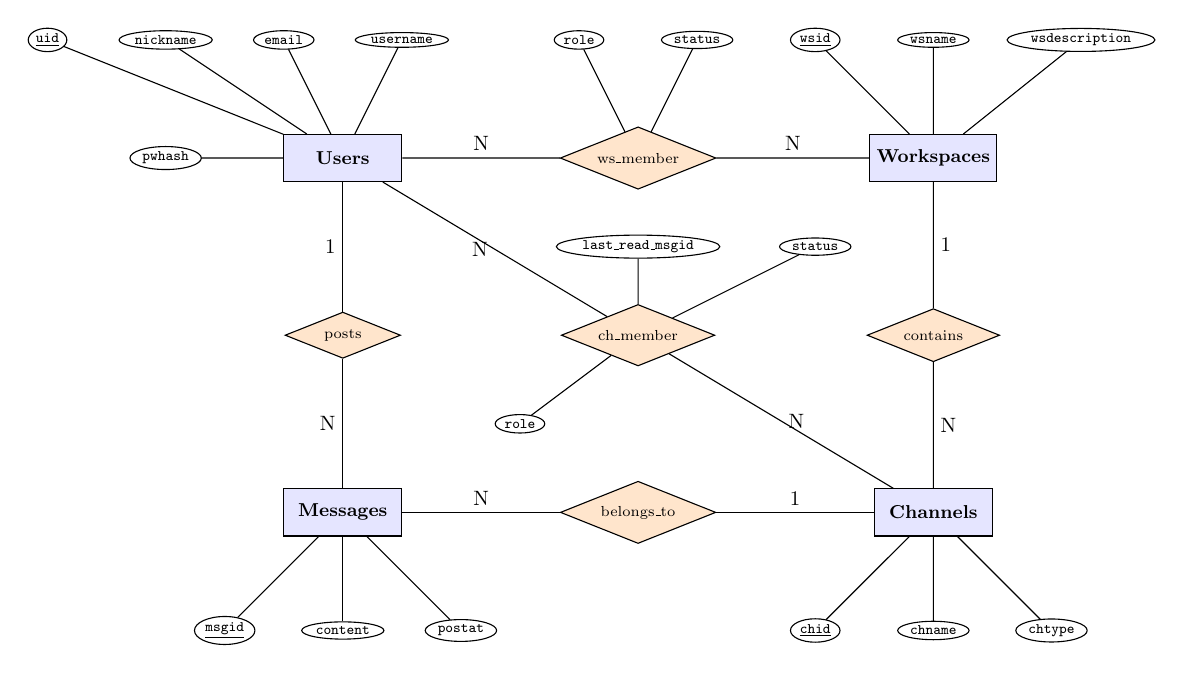
\begin{tikzpicture}[
    entity/.style={rectangle, draw, fill=blue!10, minimum width=2cm, minimum height=0.8cm, font=\small\bfseries},
    relationship/.style={diamond, draw, fill=orange!20, aspect=2.5, font=\scriptsize},
    attr/.style={ellipse, draw, fill=white, inner sep=1pt, font=\scriptsize\ttfamily},
    >=Stealth,
    scale=0.75, transform shape
]

% Row 1: Entities
\node[entity] (user) at (0, 6) {Users};
\node[entity] (workspace) at (10, 6) {Workspaces};
\node[entity] (channel) at (10, 0) {Channels};
\node[entity] (message) at (0, 0) {Messages};

% Row 2: Relationships (links in the middle)
\node[relationship] (wm) at (5, 6) {ws\_member};
\node[relationship] (cm) at (5, 3) {ch\_member};
\node[relationship] (posts) at (0, 3) {posts};
\node[relationship] (contains) at (10, 3) {contains};
\node[relationship] (belongsto) at (5, 0) {belongs\_to};

% User attributes (above and left)
\node[attr] (uuid) at (-5, 8) {\underline{uid}};
\node[attr] (uemail) at (-1, 8) {email};
\node[attr] (uname) at (1, 8) {username};
\node[attr] (unick) at (-3, 8) {nickname};
\node[attr] (upw) at (-3, 6) {pwhash};

% Workspace attributes (above and right)
\node[attr] (wsid) at (8, 8) {\underline{wsid}};
\node[attr] (wsname) at (10, 8) {wsname};
\node[attr] (wsdesc) at (12.5, 8) {wsdescription};

% Channel attributes (below and right)
\node[attr] (chid) at (8, -2) {\underline{chid}};
\node[attr] (chname) at (10, -2) {chname};
\node[attr] (chtype) at (12, -2) {chtype};

% Message attributes (below and left)
\node[attr] (msgid) at (-2, -2) {\underline{msgid}};
\node[attr] (content) at (0, -2) {content};
\node[attr] (postat) at (2, -2) {postat};

% ws_member attributes (above the diamond)
\node[attr] (wmrole) at (4, 8) {role};
\node[attr] (wmstatus) at (6, 8) {status};

% ch_member attributes (sides of the diamond)
\node[attr] (cmrole) at (3, 1.5) {role};
\node[attr] (cmstatus) at (8, 4.5) {status};
\node[attr] (cmread) at (5, 4.5) {last\_read\_msgid};

% Edges: User attributes
\draw (user) -- (uuid);
\draw (user) -- (uemail);
\draw (user) -- (uname);
\draw (user) -- (unick);
\draw (user) -- (upw);

% Edges: Workspace attributes
\draw (workspace) -- (wsid);
\draw (workspace) -- (wsname);
\draw (workspace) -- (wsdesc);

% Edges: Channel attributes
\draw (channel) -- (chid);
\draw (channel) -- (chname);
\draw (channel) -- (chtype);

% Edges: Message attributes
\draw (message) -- (msgid);
\draw (message) -- (content);
\draw (message) -- (postat);

% Edges: Relationship attributes
\draw (wm) -- (wmrole);
\draw (wm) -- (wmstatus);
\draw (cm) -- (cmrole);
\draw (cm) -- (cmstatus);
\draw (cm) -- (cmread);

% Edges: Entity-Relationship connections
\draw (user) -- node[above] {N} (wm);
\draw (workspace) -- node[above] {N} (wm);
\draw (user) -- node[left] {N} (cm);
\draw (channel) -- node[right] {N} (cm);
\draw (user) -- node[left] {1} (posts);
\draw (posts) -- node[left] {N} (message);
\draw (workspace) -- node[right] {1} (contains);
\draw (contains) -- node[right] {N} (channel);
\draw (message) -- node[above] {N} (belongsto);
\draw (belongsto) -- node[above] {1} (channel);

\end{tikzpicture}
\end{center}

\subsection{Relational Schema}

The ER diagram translates into the following six relations:

\begin{enumerate}
\item \textbf{users}(\underline{uid}, email, username, nickname, pwhash, createdat, updatedat)
\begin{itemize}
\item email is \texttt{UNIQUE NOT NULL}
\end{itemize}

\item \textbf{workspaces}(\underline{wsid}, wsname, wsdescription, createdat, updatedat)

\item \textbf{workspace\_members}(\underline{wsid}, \underline{uid}, role, status, createdat, updatedat)
    \begin{itemize}
        \item wsid $\rightarrow$ workspaces(wsid)
        \item uid $\rightarrow$ users(uid)
        \item role $\in$ \{creator, admin, member\}
        \item status $\in$ \{pending, accepted, rejected\}
    \end{itemize}

\item \textbf{channels}(\underline{chid}, wsid, chname, chtype, createdat, updatedat)
    \begin{itemize}
        \item wsid $\rightarrow$ workspaces(wsid)
        \item chtype $\in$ \{public, private, direct\}
    \end{itemize}

\item \textbf{channel\_members}(\underline{chid}, \underline{uid}, role, status, last\_read\_msgid, createdat, updatedat)
    \begin{itemize}
        \item chid $\rightarrow$ channels(chid)
        \item uid $\rightarrow$ users(uid)
        \item role $\in$ \{creator, member\}
        \item status $\in$ \{pending, accepted, rejected\}
    \end{itemize}

\item \textbf{messages}(\underline{msgid}, chid, uid, content, postat)
    \begin{itemize}
        \item chid $\rightarrow$ channels(chid)
        \item uid $\rightarrow$ users(uid)
    \end{itemize}

\end{enumerate}


\subsection{Design Assumptions}

\begin{itemize}
\item \textbf{A surrogate \texttt{uid} is used as the primary key for users}, rather than \texttt{email}. This allows users to change their email address without cascading updates across all foreign keys. The \texttt{email} column is constrained as \texttt{UNIQUE NOT NULL}.
\item \textbf{Creator is stored in membership tables, not in workspace/channel tables.} The creator is the first member inserted with role = \texttt{'creator'}. As specified in the requirements, the creator is treated as the initial administrator; query~(3) therefore includes both \texttt{'creator'} and \texttt{'admin'} roles when listing administrators. Storing the creator as a role avoids redundancy and simplifies queries.
\item \textbf{Invitations are tracked via the \texttt{status} field}, not as a separate entity. When a user is invited to a workspace or channel, a membership record is inserted with \texttt{status = 'pending'}. Upon acceptance, it is updated to \texttt{'accepted'}, and users may also explicitly decline an invitation by setting \texttt{'rejected'}. This design supports richer user interaction without introducing a separate invitations table.
\item \textbf{Public channels are visible to all workspace members but still require explicit membership.} Users are not automatically added upon channel creation; instead, they must choose to join. When a user joins a public channel, a record is inserted into \texttt{channel\_members} with \texttt{status = 'accepted'}, granting access to the channel's messages.
\item \textbf{Passwords are stored as SHA-256 hashes.} The \texttt{pwhash} field stores a hashed password rather than plaintext for security.
\item \textbf{Timestamps are recorded for all actions.} All tables include \texttt{createdat} and \texttt{updatedat} fields (messages use \texttt{postat} instead). While \texttt{updatedat} is not exercised by the required queries, it is included to support features such as profile edits, role changes, and invitation acceptance tracking.
\item \textbf{Member removal} is supported by deleting the corresponding row from \texttt{workspace\_members} or \texttt{channel\_members}. No soft-delete flag is needed since the membership record itself represents the relationship.
\item \textbf{Direct channels are limited to two members}, enforced at the application level rather than via a database constraint, since a \texttt{CHECK} on member count would require a trigger.
\item \textbf{Message read state is tracked at the channel level.} Each \texttt{channel\_members} record includes a \texttt{last\_read\_msgid} attribute, which stores the most recent message viewed by the user in that channel.
\item \textbf{Access control is enforced at the application level}, not through database permissions or views, as specified in the project requirements.
\end{itemize}

\subsection{Application-Level Enforcement}

The following constraints are enforced by the web application rather than the database, either because SQL \texttt{CHECK} constraints cannot express them without triggers, or because they involve session state:

\begin{itemize}
\item \textbf{Direct channel membership limit.} The application ensures that exactly two users are associated with a direct channel at creation time.
\item \textbf{Workspace invitation authority.} Only users with \texttt{role IN ('creator', 'admin')} in \texttt{workspace\_members} are permitted to insert new membership records for other users.
\item \textbf{Private channel invitation authority.} Only the channel creator (\texttt{role = 'creator'} in \texttt{channel\_members}) may invite additional users to a private channel.
\item \textbf{Session identification.} Each HTTP request includes a session cookie identifying the logged-in user \texttt{uid}. The application resolves this identity before executing any query.
\item \textbf{Public channel join eligibility.} Before inserting a \texttt{channel\_members} row for a public channel, the application verifies that the user has \texttt{status = 'accepted'} in the corresponding \texttt{workspace\_members} relation.
\end{itemize}


\subsection{Space Efficiency}

\begin{itemize}
    \item \textbf{No redundant creator columns.} Instead of storing a separate \texttt{creator\_uid} in the \texttt{workspaces} and \texttt{channels} tables, we encode the creator as a membership record with \texttt{role = 'creator'}.
    \item \textbf{Composite primary keys} on \texttt{workspace\_members} and \texttt{channel\_members} eliminate the need for surrogate ID columns in junction tables.
    \item \textbf{\texttt{VARCHAR} with appropriate limits} is used instead of fixed-length \texttt{CHAR} fields, so shorter values do not waste space.
    \item \textbf{\texttt{SERIAL} auto-increment} is used for \texttt{uid}, \texttt{wsid}, \texttt{chid}, and \texttt{msgid} (4-byte integers), which is more compact than UUIDs.
    \item \textbf{No separate invitations table.} The \texttt{status} field on membership tables tracks invitation state in-place, avoiding an extra table and the joins it would require.
\end{itemize}



\newpage
\section{Schema Creation}
\label{sec:creation}

The following SQL creates the schema in PostgreSQL with all key, foreign key, and check constraints:

\begin{lstlisting}
CREATE TABLE users (
    uid         SERIAL       PRIMARY KEY,
    email       VARCHAR(255) NOT NULL UNIQUE,
    username    VARCHAR(50)  NOT NULL,
    nickname    VARCHAR(50),
    pwhash      VARCHAR(255) NOT NULL,
    createdat   TIMESTAMP    NOT NULL DEFAULT CURRENT_TIMESTAMP,
    updatedat   TIMESTAMP    NOT NULL DEFAULT CURRENT_TIMESTAMP
);

CREATE TABLE workspaces (
    wsid        SERIAL       PRIMARY KEY,
    wsname      VARCHAR(100) NOT NULL,
    wsdescription TEXT,
    createdat   TIMESTAMP    NOT NULL DEFAULT CURRENT_TIMESTAMP,
    updatedat   TIMESTAMP    NOT NULL DEFAULT CURRENT_TIMESTAMP
);

CREATE TABLE workspace_members (
    wsid        INT          NOT NULL REFERENCES workspaces(wsid),
    uid         INT          NOT NULL REFERENCES users(uid),
    role        VARCHAR(10)  NOT NULL CHECK (role IN ('creator', 'admin', 'member')),
    status      VARCHAR(10)  NOT NULL CHECK (status IN ('pending', 'accepted', 'rejected'))
                             DEFAULT 'pending',
    createdat   TIMESTAMP    NOT NULL DEFAULT CURRENT_TIMESTAMP,
    updatedat   TIMESTAMP    NOT NULL DEFAULT CURRENT_TIMESTAMP,
    PRIMARY KEY (wsid, uid)
);

CREATE TABLE channels (
    chid        SERIAL       PRIMARY KEY,
    wsid        INT          NOT NULL REFERENCES workspaces(wsid),
    chname      VARCHAR(100),
    chtype      VARCHAR(10)  NOT NULL CHECK (chtype IN ('public', 'private', 'direct')),
    createdat   TIMESTAMP    NOT NULL DEFAULT CURRENT_TIMESTAMP,
    updatedat   TIMESTAMP    NOT NULL DEFAULT CURRENT_TIMESTAMP
);

CREATE TABLE channel_members (
    chid        INT          NOT NULL REFERENCES channels(chid),
    uid         INT          NOT NULL REFERENCES users(uid),
    role        VARCHAR(10)  NOT NULL CHECK (role IN ('creator', 'member')),
    status      VARCHAR(10)  NOT NULL CHECK (status IN ('pending', 'accepted', 'rejected'))
                             DEFAULT 'pending',
    last_read_msgid INT,
    createdat   TIMESTAMP    NOT NULL DEFAULT CURRENT_TIMESTAMP,
    updatedat   TIMESTAMP    NOT NULL DEFAULT CURRENT_TIMESTAMP,
    PRIMARY KEY (chid, uid)
);

CREATE TABLE messages (
    msgid       SERIAL       PRIMARY KEY,
    chid        INT          NOT NULL REFERENCES channels(chid),
    uid         INT          NOT NULL REFERENCES users(uid),
    content     TEXT         NOT NULL,
    postat      TIMESTAMP    NOT NULL DEFAULT CURRENT_TIMESTAMP
);
\end{lstlisting}

\newpage
\section{Queries}
\label{sec:queries}

\subsection{(1) Create a new user account}

\begin{lstlisting}
CREATE OR REPLACE PROCEDURE create_user(
    p_email    VARCHAR,
    p_username VARCHAR,
    p_nickname VARCHAR,
    p_pwhash   VARCHAR
)
LANGUAGE SQL
AS $$
    INSERT INTO users (email, username, nickname, pwhash)
    VALUES (p_email, p_username, p_nickname, p_pwhash);
$$;

-- Example call:
CALL create_user('gz1234@nyu.edu', 'gracezhu', 'Grace', 'a1b2c3d4e5f6');
\end{lstlisting}

\noindent\textbf{Test:} Calling with a new email succeeds and inserts a row into \texttt{users}. Calling with a duplicate email raises a unique constraint violation.

\subsection{(2) Create a new public channel (with authorization check)}

\begin{lstlisting}
CREATE OR REPLACE PROCEDURE create_public_channel(
    p_wsid    INT,
    p_uid     INT,
    p_chname  VARCHAR
)
LANGUAGE plpgsql
AS $$
DECLARE
    v_chid INT;
BEGIN
    IF NOT EXISTS (
        SELECT 1 FROM workspace_members
        WHERE wsid = p_wsid AND uid = p_uid AND status = 'accepted'
    ) THEN
        RAISE EXCEPTION 'User % is not an accepted member of workspace %',
            p_uid, p_wsid;
    END IF;
    INSERT INTO channels (wsid, chname, chtype)
    VALUES (p_wsid, p_chname, 'public')
    RETURNING chid INTO v_chid;
    INSERT INTO channel_members (chid, uid, role, status)
    VALUES (v_chid, p_uid, 'creator', 'accepted');
END;
$$;

-- Example call:
CALL create_public_channel(1, 1, 'announcements');
\end{lstlisting}

\noindent\textbf{Test:} Calling with an accepted workspace member succeeds; calling with a non-member raises an exception.

\subsection{(3) For each workspace, list all current administrators}

\begin{lstlisting}
SELECT w.wsid, w.wsname, u.email, u.username, wm.role
FROM workspaces w
JOIN workspace_members wm ON w.wsid = wm.wsid
JOIN users u ON wm.uid = u.uid
WHERE wm.role IN ('creator', 'admin') AND wm.status = 'accepted'
ORDER BY w.wsid, wm.role;
\end{lstlisting}

\noindent\textbf{Result:}
\begin{center}
\tiny
\begin{tabular}{cllll}
\toprule
wsid & wsname & email & username & role \\
\midrule
1 & CS Department & bs5678@nyu.edu & bobsmith & admin \\
1 & CS Department & az1234@nyu.edu & alicezhang & creator \\
2 & Tandon Robotics Club & cw9012@nyu.edu & carolwang & admin \\
2 & Tandon Robotics Club & bs5678@nyu.edu & bobsmith & creator \\
3 & DB Project Team & gs6789@nyu.edu & gracesun & admin \\
3 & DB Project Team & cw9012@nyu.edu & carolwang & creator \\
\bottomrule
\end{tabular}
\end{center}

\subsection{(4) Pending invitations per public channel (older than 5 days)}

\begin{lstlisting}
SELECT c.chid, c.chname, COUNT(cm.uid) AS pending_count
FROM channels c
LEFT JOIN channel_members cm ON c.chid = cm.chid
    AND cm.status = 'pending'
    AND cm.createdat < CURRENT_TIMESTAMP - INTERVAL '5 days'
WHERE c.wsid = 1 AND c.chtype = 'public'
GROUP BY c.chid, c.chname
ORDER BY c.chid;
\end{lstlisting}

\noindent\textbf{Result:}
\begin{center}
\tiny
\begin{tabular}{clc}
\toprule
chid & chname & pending\_count \\
\midrule
1 & general & 1 \\
4 & research & 0 \\
\bottomrule
\end{tabular}
\end{center}

\subsection{(5) List all messages in a channel in chronological order}

\begin{lstlisting}
CREATE OR REPLACE FUNCTION list_channel_messages(p_chid INT)
RETURNS TABLE (
    msgid INT, email VARCHAR, username VARCHAR,
    content TEXT, postat TIMESTAMP
)
LANGUAGE SQL
AS $$
    SELECT m.msgid, u.email, u.username, m.content, m.postat
    FROM messages m
    JOIN users u ON m.uid = u.uid
    WHERE m.chid = p_chid
    ORDER BY m.postat ASC;
$$;

-- Example call:
SELECT * FROM list_channel_messages(1);
\end{lstlisting}

\noindent\textbf{Result (channel 1, \#general):}
\begin{center}
\tiny
\begin{tabular}{cllll}
\toprule
msgid & email & username & content & postat \\
\midrule
1 & az1234@nyu.edu & alicezhang & Welcome to the CS Department workspace! & 2026-04-01 09:00 \\
2 & bs5678@nyu.edu & bobsmith & Thanks Alice! Excited to be here. & 2026-04-01 09:05 \\
3 & cw9012@nyu.edu & carolwang & Is the new curriculum perpendicular\ldots & 2026-04-01 09:10 \\
4 & az1234@nyu.edu & alicezhang & Not exactly perpendicular, but quite different. & 2026-04-01 09:15 \\
5 & gs6789@nyu.edu & gracesun & Hi everyone! Just joined the department. & 2026-04-01 09:20 \\
\bottomrule
\end{tabular}
\end{center}

\newpage
\subsection{(6) List all messages posted by a particular user}

\begin{lstlisting}
SELECT m.msgid, c.chname, m.content, m.postat
FROM messages m
JOIN channels c ON m.chid = c.chid
WHERE m.uid = 1  -- Alice
ORDER BY m.postat DESC;
\end{lstlisting}

\noindent\textbf{Result (Alice, uid=1):} Returns all messages Alice has posted across \#general, \#hiring-committee, DM with Bob, and \#research, ordered most recent first.

\subsection{(7) Search accessible messages by keyword}

\begin{lstlisting}
CREATE OR REPLACE FUNCTION search_accessible_messages(
    p_uid INT, p_keyword VARCHAR
)
RETURNS TABLE (
    msgid INT, chname VARCHAR, author VARCHAR,
    content TEXT, postat TIMESTAMP
) LANGUAGE SQL AS $$
    SELECT m.msgid, c.chname, u.email AS author,
           m.content, m.postat
    FROM messages m
    JOIN channels c ON m.chid = c.chid
    JOIN users u ON m.uid = u.uid
    JOIN channel_members cm ON c.chid = cm.chid AND cm.uid = p_uid
    JOIN workspace_members wm
      ON c.wsid = wm.wsid AND wm.uid = p_uid
    WHERE cm.status = 'accepted'
      AND wm.status = 'accepted'
      AND m.content ILIKE '%' || p_keyword || '%'
    ORDER BY m.postat DESC;
$$;
-- Example call:
SELECT * FROM search_accessible_messages(1, 'perpendicular');
\end{lstlisting}

\noindent\textbf{Result:}
\begin{center}
\tiny
\begin{tabular}{cllll}
\toprule
msgid & chname & author & content & postat \\
\midrule
4 & general & az1234@nyu.edu & Not exactly perpendicular, but quite different. & 2026-04-01 09:15 \\
3 & general & cw9012@nyu.edu & Is the new curriculum perpendicular\ldots & 2026-04-01 09:10 \\
\bottomrule
\end{tabular}
\end{center}

\noindent\textbf{Access control verification:}
\begin{enumerate}
    \item \textbf{Alice (uid=1):} Accepted in WS1 and channel \#general $\Rightarrow$ 2 results (plus 1 from \#research). \checkmark
    \item \textbf{Dave (uid=4):} Pending in channel \#general but accepted in WS2 \#events $\Rightarrow$ only the \#events match returned. \checkmark
    \item \textbf{Eve (uid=5):} Pending workspace invitation $\Rightarrow$ 0 results. \checkmark
\end{enumerate}

\newpage
\section{Test Data}
\label{sec:testdata}

The test dataset consists of \textbf{8 users}, \textbf{3 workspaces}, \textbf{11 channels} (covering public, private, and direct types), and \textbf{over 60 messages}.

\subsection{Data Structure Overview}

\begin{itemize}
    \item \textbf{8 users} span three workspaces with overlapping membership. Bob, Carol, and Dave appear in multiple workspaces, testing cross-workspace queries.
    \item \textbf{3 workspaces:} CS Department (academic), Tandon Robotics Club (extracurricular), DB Project Team (course project). This variety creates realistic usage patterns.
    \item \textbf{Role diversity:} Alice is a workspace creator (WS1) and channel creator. Bob is both a workspace creator (WS2) and an admin (WS1). Carol is a workspace creator (WS3) and admin (WS2). This tests query~(3).
    \item \textbf{Pending invitations:} Eve has a pending workspace invite; Dave and Frank have pending channel invites older than 5 days. This tests query~(4).
    \item \textbf{60+ messages} are distributed across all channels with natural conversation patterns. Multiple messages contain the keyword ``perpendicular'' across different workspaces, testing query~(7)'s keyword search with access control.
    \item \textbf{Diverse channel types} per workspace: each workspace has public channels, and at least one private channel or direct message channel.
\end{itemize}

\subsection{Sample Data Snapshot}

\noindent\textbf{Users:}
\begin{center}
\tiny
\begin{tabular}{clll}
\toprule
uid & email & username & nickname \\
\midrule
1 & az1234@nyu.edu & alicezhang & Alice \\
2 & bs5678@nyu.edu & bobsmith & Bob \\
3 & cw9012@nyu.edu & carolwang & Carol \\
4 & dj3456@nyu.edu & davejohnson & Dave \\
5 & ec7890@nyu.edu & evechen & Eve \\
6 & fl2345@nyu.edu & frankli & Frank \\
7 & gs6789@nyu.edu & gracesun & Grace \\
8 & hk1234@nyu.edu & henrykim & Henry \\
\bottomrule
\end{tabular}
\end{center}

\noindent\textbf{Workspace Members} (excerpt):
\begin{center}
\tiny
\begin{tabular}{cclcc}
\toprule
wsid & uid & role & status & notes \\
\midrule
1 & 1 & creator & accepted & Alice created CS Dept \\
1 & 2 & admin & accepted & Bob is admin \\
1 & 5 & member & pending & Eve invited, not joined \\
2 & 2 & creator & accepted & Bob created Robotics \\
2 & 1 & member & pending & Alice invited, not joined \\
3 & 3 & creator & accepted & Carol created DB Project \\
3 & 7 & admin & accepted & Grace is admin \\
\bottomrule
\end{tabular}
\end{center}


%% ================================================================
%%  PART 2 — WEB APPLICATION
%% ================================================================

\newpage
\section{System Architecture}
\label{sec:arch}

\subsection{Technology Stack}

\begin{itemize}
    \item \textbf{Backend:} Django 5.2 (Python) --- serves the API via a single RPC endpoint
    \item \textbf{Database:} PostgreSQL 15 --- all queries use raw SQL (no ORM)
    \item \textbf{Frontend:} React 18 with Tailwind CSS --- single-page application
    \item \textbf{Deployment:} Docker Compose --- PostgreSQL container + Django container
\end{itemize}

\subsection{Architecture Diagram}

\begin{center}
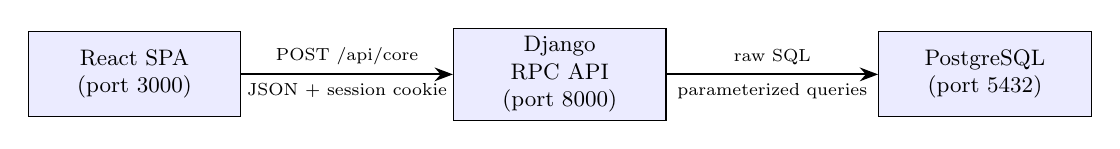
\begin{tikzpicture}[
    box/.style={rectangle, draw, fill=blue!8, minimum width=3cm, minimum height=1.2cm, font=\small, align=center},
    arr/.style={->, thick, >=Stealth},
    scale=0.9, transform shape
]
\node[box] (browser) at (0, 0) {React SPA\\(port 3000)};
\node[box] (django) at (6, 0) {Django\\RPC API\\(port 8000)};
\node[box] (pg) at (12, 0) {PostgreSQL\\(port 5432)};

\draw[arr] (browser) -- node[above, font=\scriptsize] {POST /api/core} node[below, font=\scriptsize] {JSON + session cookie} (django);
\draw[arr] (django) -- node[above, font=\scriptsize] {raw SQL} node[below, font=\scriptsize] {parameterized queries} (pg);
\end{tikzpicture}
\end{center}

\subsection{RPC API Design}

Rather than a RESTful API with multiple endpoints and HTTP verbs, we use a single \textbf{Remote Procedure Call (RPC)} endpoint at \texttt{POST /api/core}. Every request contains a JSON body:

\begin{lstlisting}[language=Python]
{"function": "function_name", "args": [], "kwargs": {}}
\end{lstlisting}

The server dispatches to the named Python function, which executes the corresponding SQL queries and returns the result as JSON. This approach was chosen for simplicity --- the backend is a single \texttt{views.py} file with a function registry, making it easy to add new operations without creating new URL patterns or view classes.

\subsection{Available API Functions}

\begin{center}
\small
\begin{tabular}{ll}
\toprule
Category & Functions \\
\midrule
Auth & \texttt{register}, \texttt{login}, \texttt{logout}, \texttt{me} \\
Workspaces & \texttt{get\_workspaces}, \texttt{create\_workspace}, \texttt{delete\_workspace} \\
 & \texttt{get\_workspace\_members}, \texttt{invite\_to\_workspace} \\
 & \texttt{respond\_workspace\_invite}, \texttt{update\_workspace\_member}, \texttt{leave\_workspace} \\
Channels & \texttt{get\_channels}, \texttt{create\_channel}, \texttt{delete\_channel} \\
 & \texttt{get\_channel\_members}, \texttt{invite\_to\_channel}, \texttt{respond\_channel\_invite} \\
 & \texttt{join\_channel}, \texttt{leave\_channel}, \texttt{get\_public\_channels} \\
Messages & \texttt{get\_messages}, \texttt{send\_message}, \texttt{search\_messages}, \texttt{get\_user\_messages} \\
Users & \texttt{search\_users} \\
Admin & \texttt{initialize} \\
\bottomrule
\end{tabular}
\end{center}


\newpage
\section{Implementation Details}
\label{sec:impl}

\subsection{Backend Implementation}

The entire backend is contained in \texttt{DBProject/views.py}. Key implementation choices:

\begin{itemize}
    \item \textbf{Raw SQL only.} Every database operation uses \texttt{connection.cursor()} and parameterized SQL queries. Django's ORM is not used, in compliance with the course requirement. For example, the login function:
\end{itemize}

\begin{lstlisting}[language=Python]
def login(request, username, password):
    with connection.cursor() as c:
        c.execute(
            "SELECT uid, email, username, nickname, pwhash "
            "FROM users WHERE username = %s",
            [username],
        )
        user = _dictfetchone(c)
    if not user or user["pwhash"] != _hash(password):
        return {"error": "invalid credentials"}
    request.session["uid"] = user["uid"]
    return user
\end{lstlisting}

\begin{itemize}
    \item \textbf{Session-based authentication.} Django's built-in session framework stores the user's \texttt{uid} in a server-side session. A session cookie (\texttt{sessionid}) is sent to the browser. Every protected function checks \texttt{request.session.get("uid")} before proceeding.
    \item \textbf{Password hashing.} Passwords are hashed with SHA-256 before storage. The hash comparison is performed in Python, not in SQL.
    \item \textbf{Authorization checks.} Operations like \texttt{invite\_to\_workspace} first query the caller's role and verify it is \texttt{'creator'} or \texttt{'admin'} before proceeding.
\end{itemize}

\subsection{Frontend Implementation}

The frontend is a React single-page application with the following component hierarchy:

\begin{itemize}
    \item \texttt{App.js} --- top-level routing (login vs.\ chat page)
    \item \texttt{LoginPage.js} / \texttt{RegisterPage.js} --- authentication forms
    \item \texttt{ChatPage.js} --- main layout with state management
    \begin{itemize}
        \item \texttt{WorkspaceList.js} --- left sidebar listing workspaces
        \item \texttt{ChannelList.js} --- second sidebar listing channels
        \item \texttt{ChatWindow.js} --- message display and input area
        \item \texttt{Inbox.js} --- dropdown for pending invitations
        \item \texttt{SearchModal.js} --- keyword search across all accessible messages
        \item Various modals: \texttt{CreateWorkspaceModal}, \texttt{CreateChannelModal}, \texttt{WorkspaceMembersModal}, \texttt{ChannelSettingsModal}, \texttt{DiscoverChannelsModal}
    \end{itemize}
\end{itemize}

All API calls go through \texttt{services/api.js}, which wraps the RPC protocol and includes \texttt{credentials: "include"} for session cookie handling across the cross-origin boundary (React on port 3000, Django on port 8000).

\subsection{Key Features}

\begin{enumerate}
    \item \textbf{User registration and login} --- users create accounts with email, username, nickname, and password. Sessions persist across page refreshes via the \texttt{me} endpoint.
    \item \textbf{Workspace management} --- create workspaces, invite members (by searching usernames), promote/demote admins, remove members, leave or delete workspaces.
    \item \textbf{Channel types} --- public (discoverable, self-join), private (invite-only), and direct messages (two-person).
    \item \textbf{Messaging} --- send and view messages in real-time within a channel. Messages display chronologically with sender name and timestamp.
    \item \textbf{Invitation inbox} --- pending workspace and channel invitations appear in a dropdown; users can accept or reject each.
    \item \textbf{Public channel discovery} --- a ``Browse'' button lists public channels in the current workspace that the user has not yet joined. One-click join.
    \item \textbf{Message search} --- a search modal allows users to search for messages by keyword across all channels they have access to. Results show the channel name, author, content, and timestamp.
\end{enumerate}


\newpage
\section{Security}
\label{sec:security}

\subsection{SQL Injection Prevention}

All database queries use \textbf{parameterized queries} with \texttt{\%s} placeholders. User-supplied values are never concatenated into SQL strings. Django's database adapter passes parameters separately to PostgreSQL, which treats them as data, not executable SQL.

\begin{lstlisting}[language=Python]
# Safe: parameterized query
c.execute(
    "SELECT uid, email, username, nickname FROM users "
    "WHERE username ILIKE %s OR email ILIKE %s LIMIT 20",
    [f"%{query}%", f"%{query}%"],
)
\end{lstlisting}

The stored procedures defined in \texttt{query.sql} (e.g., \texttt{create\_user}, \texttt{create\_public\_channel}) also use parameterized inputs, providing an additional layer of protection when called directly.

\subsection{Cross-Site Scripting (XSS) Prevention}

The frontend uses React, which \textbf{automatically escapes all content rendered in JSX}. When a variable is placed inside curly braces (\texttt{\{msg.content\}}), React converts special characters (\texttt{<}, \texttt{>}, \texttt{\&}, \texttt{"}, \texttt{'}) to their HTML entity equivalents before inserting them into the DOM. This prevents any user-supplied content (message text, usernames, channel names) from being interpreted as HTML or JavaScript.

We do not use \texttt{dangerouslySetInnerHTML} anywhere in the codebase, so there is no bypass of React's built-in XSS protection.

\subsection{Cross-Site Request Forgery (CSRF)}

The RPC endpoint uses \texttt{@csrf\_exempt} because the frontend is a separate React application that communicates via JSON \texttt{POST} requests with session cookies. CSRF protection is less critical here because:
\begin{enumerate}
    \item The endpoint only accepts \texttt{POST} with a \texttt{Content-Type: application/json} header.
    \item Browsers enforce CORS preflight checks for cross-origin JSON requests, preventing third-party sites from forging requests with the correct content type.
    \item Django's \texttt{CORS\_ALLOWED\_ORIGINS} is configured to only allow the frontend's origin.
\end{enumerate}

\subsection{Concurrency and Transaction Safety}
\label{sec:concurrency}

Multi-step database operations are wrapped in \texttt{transaction.atomic()} to ensure atomicity. If any step fails, the entire transaction is rolled back, preventing partial state changes.

The following operations use explicit transactions:

\begin{itemize}
    \item \texttt{create\_workspace} --- inserts into \texttt{workspaces} and \texttt{workspace\_members}
    \item \texttt{create\_channel} --- checks membership, inserts into \texttt{channels} and \texttt{channel\_members}
    \item \texttt{delete\_channel} --- deletes from \texttt{messages}, \texttt{channel\_members}, and \texttt{channels}
    \item \texttt{delete\_workspace} --- cascading delete across five tables
    \item \texttt{invite\_to\_workspace} --- checks role, then inserts invitation
    \item \texttt{update\_workspace\_member} --- checks role, then modifies/removes member
    \item \texttt{initialize} --- drops and recreates all tables with test data
\end{itemize}

Example:

\begin{lstlisting}[language=Python]
def delete_workspace(request, wsid):
    uid = request.session.get("uid")
    if not uid:
        return {"error": "not logged in"}
    with transaction.atomic():
        with connection.cursor() as c:
            c.execute("SELECT role FROM workspace_members "
                      "WHERE wsid=%s AND uid=%s", [wsid, uid])
            row = _dictfetchone(c)
            if not row or row["role"] != "creator":
                return {"error": "only the workspace creator can delete it"}
            c.execute("DELETE FROM messages WHERE chid IN "
                      "(SELECT chid FROM channels WHERE wsid=%s)", [wsid])
            c.execute("DELETE FROM channel_members WHERE chid IN "
                      "(SELECT chid FROM channels WHERE wsid=%s)", [wsid])
            c.execute("DELETE FROM channels WHERE wsid=%s", [wsid])
            c.execute("DELETE FROM workspace_members WHERE wsid=%s", [wsid])
            c.execute("DELETE FROM workspaces WHERE wsid=%s", [wsid])
    return {"ok": True}
\end{lstlisting}

PostgreSQL's default isolation level (\texttt{READ COMMITTED}) ensures that concurrent sessions do not see uncommitted changes from other transactions. This prevents issues such as:

\begin{itemize}
    \item A user reading messages from a channel that is being deleted by another user.
    \item Two users simultaneously creating a workspace and both getting the same \texttt{wsid}.
    \item An invitation being accepted while the workspace is being deleted.
\end{itemize}

Single-statement operations (e.g., \texttt{send\_message}, \texttt{get\_messages}) run in Django's default autocommit mode, which is safe because a single SQL statement is inherently atomic in PostgreSQL.


\newpage
\section{User Guide}
\label{sec:guide}

\subsection{Getting Started}

\begin{enumerate}
    \item \textbf{Start the system:} Run \texttt{docker compose up --build} from the project root.
    \item \textbf{Initialize the database:} Open \texttt{http://localhost:8000} and click the \textbf{Initialize} button to create tables and load test data.
    \item \textbf{Open the frontend:} Navigate to \texttt{http://localhost:3000}.
    \item \textbf{Log in or register:} Use a test account (e.g., \texttt{alicezhang} / \texttt{alice123}) or create a new account.
\end{enumerate}

\subsection{Main Interface}

The main interface consists of three panels:
\begin{itemize}
    \item \textbf{Left sidebar (purple):} Lists your workspaces. Click to select. The ``+'' button creates a new workspace.
    \item \textbf{Middle sidebar (gray):} Lists channels in the selected workspace. Click to open. Includes buttons for creating channels and browsing public channels.
    \item \textbf{Main area (white):} Displays messages in the selected channel. Type a message and click Send or press Enter.
\end{itemize}

\subsection{Top Bar Actions}

\begin{itemize}
    \item \textbf{Search:} Opens a modal where you can search for messages by keyword across all your accessible channels. Results show the channel name, author, content, and timestamp.
    \item \textbf{Inbox:} Shows pending workspace and channel invitations. Accept or reject each with a single click.
    \item \textbf{Logout:} Ends the session and returns to the login page.
\end{itemize}

\subsection{Workspace Management}

Click ``Members \& settings'' at the bottom of the workspace sidebar to:
\begin{itemize}
    \item View all workspace members and their roles
    \item Invite new members by searching usernames (creator/admin only)
    \item Promote or demote members to/from admin (creator/admin only)
    \item Remove members (creator/admin only)
    \item Leave the workspace (non-creators)
    \item Delete the workspace (creator only --- cascades to all channels and messages)
\end{itemize}

\subsection{Channel Management}

Click ``Channel settings'' at the bottom of the channel sidebar to:
\begin{itemize}
    \item View channel members
    \item Add members from the workspace (channel creator only)
    \item Leave the channel
    \item Delete the channel (channel creator only)
\end{itemize}


\newpage
\section{Session Logs}
\label{sec:session}

Below are representative session logs demonstrating the core functionality of the system. Each log shows the API calls made and the system's responses.

\subsection{Session 1: Registration and Workspace Setup}

\begin{enumerate}
    \item User opens the registration page and creates an account:
    \begin{itemize}
        \item \texttt{register(email="jd1234@nyu.edu", username="janedoe", nickname="Jane", password="pass123")}
        \item Response: \texttt{\{uid: 9, email: "jd1234@nyu.edu", username: "janedoe"\}}
    \end{itemize}

    \item User creates a new workspace:
    \begin{itemize}
        \item \texttt{create\_workspace(wsname="Study Group", wsdescription="Finals prep")}
        \item Response: \texttt{\{wsid: 4, wsname: "Study Group"\}}
    \end{itemize}

    \item User creates a public channel in the workspace:
    \begin{itemize}
        \item \texttt{create\_channel(wsid=4, chname="algorithms", chtype="public")}
        \item Response: \texttt{\{chid: 12, chname: "algorithms", chtype: "public"\}}
    \end{itemize}

    \item User sends a message:
    \begin{itemize}
        \item \texttt{send\_message(chid=12, content="Who is ready for the algorithms final?")}
        \item Response: \texttt{\{msgid: 64, postat: "2026-04-24T10:30:00"\}}
    \end{itemize}
\end{enumerate}

\subsection{Session 2: Invitations and Collaboration}

\begin{enumerate}
    \item Alice logs in and checks her inbox:
    \begin{itemize}
        \item \texttt{login(username="alicezhang", password="alice123")}
        \item \texttt{get\_invitations()} $\Rightarrow$ \texttt{[\{type: "workspace", id: 2, name: "Tandon Robotics Club"\}]}
    \end{itemize}

    \item Alice accepts the workspace invitation:
    \begin{itemize}
        \item \texttt{respond\_workspace\_invite(wsid=2, accept=true)}
        \item Alice can now see channels in the Robotics Club workspace.
    \end{itemize}

    \item Alice searches for messages containing ``robotics'':
    \begin{itemize}
        \item \texttt{search\_messages(keyword="robotics")} $\Rightarrow$ Returns results from \#events in WS2 (now accessible after accepting the invite).
    \end{itemize}
\end{enumerate}

\subsection{Session 3: Admin Operations}

\begin{enumerate}
    \item Bob logs in and manages the CS Department workspace:
    \begin{itemize}
        \item \texttt{login(username="bobsmith", password="bob456")}
        \item \texttt{get\_workspace\_members(wsid=1)} $\Rightarrow$ Lists all members with roles.
    \end{itemize}

    \item Bob invites Eve (who has a pending invite) --- no duplicate is created due to \texttt{ON CONFLICT DO NOTHING}:
    \begin{itemize}
        \item \texttt{invite\_to\_workspace(wsid=1, invitee\_uid=5)} $\Rightarrow$ \texttt{\{ok: true\}}
    \end{itemize}

    \item Bob promotes Carol to admin:
    \begin{itemize}
        \item \texttt{update\_workspace\_member(wsid=1, target\_uid=3, role="admin")} $\Rightarrow$ \texttt{\{ok: true\}}
    \end{itemize}
\end{enumerate}


\newpage
\section{Design Decisions and Revisions for Project 2}
\label{sec:revisions}

\subsection{Schema Revisions}

The schema from Project~1 was used without structural changes. The \texttt{ON DELETE CASCADE} constraints on foreign keys were already in place, and the \texttt{status} field on membership tables naturally supports the invitation workflow required by the web interface.

\subsection{Design Decisions}

\begin{itemize}
    \item \textbf{RPC over REST.} A single endpoint simplifies both the backend (one URL pattern, one dispatcher) and the frontend (one \texttt{apiCall} helper). Adding a new feature requires only writing a new Python function and decorating it with \texttt{@rpc}.

    \item \textbf{Raw SQL only.} While Django provides a powerful ORM, we exclusively use raw SQL with parameterized queries to satisfy the course requirement and to maintain full control over the generated queries.

    \item \textbf{Session-based authentication over tokens.} Django's built-in session framework provides secure, server-side session management with minimal configuration. The session cookie is HTTP-only and signed, preventing client-side JavaScript from reading the session ID.

    \item \textbf{Application-level cascade deletes.} Although PostgreSQL supports \texttt{ON DELETE CASCADE}, the \texttt{delete\_workspace} and \texttt{delete\_channel} functions explicitly delete dependent rows in order. This gives us full control over the deletion order and allows us to wrap the entire operation in a transaction.

    \item \textbf{Docker Compose for deployment.} The entire system (Django + PostgreSQL) runs with a single \texttt{docker compose up --build} command, making it easy to set up for the demo.
\end{itemize}

\subsection{Known Limitations}

\begin{itemize}
    \item No WebSocket support --- the frontend does not receive real-time updates. Users must refresh or re-select a channel to see new messages.
    \item No message editing or deletion.
    \item No file or image uploads.
    \item Direct channel names are auto-generated as \texttt{DM - username} in the frontend but stored as \texttt{NULL} in the database.
\end{itemize}

\section{Conclusion}

We have designed and implemented \textit{snickr}, a fully functional web-based collaboration system backed by a PostgreSQL relational database. The system supports user registration, workspace and channel management, role-based access control, invitation workflows, messaging, and keyword search --- all through a clean React interface communicating with a Django backend via a single RPC endpoint.

Security measures include parameterized queries against SQL injection, React's automatic XSS escaping, session-based authentication, and transactional consistency for multi-step operations. The system can be deployed locally via Docker Compose for a live demonstration.

\end{document}
